\documentclass[10pt]{article}
\usepackage[utf8]{inputenc}\usepackage[scaled=0.92]{helvet}\renewcommand{\familydefault}{\sfdefault}
\usepackage[margin=0.75in,top=0.7in,bottom=0.7in]{geometry}
\usepackage{xcolor,booktabs,tabularx,longtable,enumitem,fancyhdr,titlesec,array,tikz,amsmath}
\usetikzlibrary{arrows.meta}
\definecolor{navy}{HTML}{1F3B5C}\definecolor{rose}{HTML}{B3412E}\definecolor{sage}{HTML}{E7F0E3}
\titleformat{\section}{\large\bfseries\color{navy}}{\thesection}{0.6em}{}[\vspace{-0.4em}{\color{navy}\titlerule}]
\titlespacing*{\section}{0pt}{1.1em}{0.5em}
\titleformat{\subsection}{\normalsize\bfseries}{}{0pt}{}\titlespacing*{\subsection}{0pt}{0.8em}{0.3em}
\pagestyle{fancy}\fancyhf{}\renewcommand{\headrulewidth}{0pt}
\fancyfoot[C]{\footnotesize Honors Physics $\cdot$ Slot 7 $\cdot$ fan-cart virtual lab $\cdot$ Mr.\ D marks this up $\cdot$ page \thepage}
\setlength{\parindent}{0pt}\setlength{\parskip}{0.35em}\setlist{itemsep=1pt,topsep=2pt,leftmargin=1.4em}
\newcolumntype{Y}{>{\raggedright\arraybackslash}X}
\renewcommand{\arraystretch}{1.18}
\begin{document}
{\LARGE\bfseries\color{navy} Slot 7 $\cdot$ The fan-cart virtual lab}\\[2pt]
{\large Honors Physics $\cdot$ Forces and Newton's Laws $\cdot$ target F5}\par
\colorbox{sage}{\parbox{\dimexpr\linewidth-2\fboxsep}{\small\textbf{The standard (T5), the top hidden band.} Say in words, with numbers from your own tables, how acceleration changes when the fan force doubles and when the mass doubles. Every student completes it. Nothing on the student page is labeled extension, challenge or optional.}}

\section{The day at a glance}
\begin{tabularx}{\linewidth}{@{}l l Y@{}}
\toprule 0:00--0:03 & Warm-up & Pre-lab on the Chromebook: three easy picture items, then one prediction. The lab door stays shut until it is done.\\
0:03 & Huddle 1 (about 8 min) & Hold screen. Mr.\ D: review, hook, first contact with the fan cart. Gives code 1.\\
0:11--0:28 & Lab in the room & Walk, take bars, read the balance, run the cart, read the speed graph, fill two tables, graph them, write the CER.\\
0:28 & Huddle 2 (about 8 min) & The most important block. Mr.\ D states what is tested, works three problems, asks three crux questions. Gives code 2.\\
0:36--0:40 & After code 2 & Graph acceleration against $1/m$. Predict and run 3 bars (1.25 kg).\\
0:40--0:42 & Exit ticket & A drawing on paper. Mr.\ D scans it by eye.\\
\bottomrule\end{tabularx}
Lab days set huddle 2 late because a lab cannot be cut off at 0:25. Code 2 is never blocked by an unfinished table. A student who is behind still gets the huddle.

\textbf{Not today.} The equation, the newton, strings, pulleys, inclines, components and friction measurement. Slot 8 turns the two patterns into the law and defines the newton. Slots 14, 19 and 20 own pulleys, systems and inclines.

\section{What this replaces, and the UBD edits to make by hand}
Mr.\ D has no fan and no cart, so the virtual lab replaces the real second-law lab at slot 7. I did not edit the UBD files. Three edits:
\begin{enumerate}
\item \textbf{Stage 1, slot 7.} Topic “Second-law lab: fan cart or hanging-mass cart” becomes “Second-law virtual lab: fan cart”. Format “Real lab” becomes “Virtual lab in the Mr.\ D's Sims room”. Hands-on days drop from seven to six (slots 1, 3, 10, 13, 15, 21). Virtual labs and sims run at slots 5, 7, 8, 16, 19 and 20.
\item \textbf{Stage 3, slot 7.} The learning event keeps its shape: vary force at fixed mass, then mass at fixed force, graph $a$ against $F$ and $a$ against $1/m$, predict a new mass, test it. “Photogates or phone video” becomes “a motion sensor drawn in the lab”.
\item \textbf{Slot 5 stays as written.} PhET Forces and Motion: Basics, F3 and F4. The angled-string, hanging-string and ramp ideas stay with slots 14, 19 and 20.
\end{enumerate}
\textbf{Why a fan cart.} The hanging-mass cart needs a string over a pulley (slot 14) and changes the mass being pulled every time the force changes (slot 19). The fan cart holds the force steady while the mass changes. No strings anywhere.

\section{Who does what}
\begin{tabularx}{\linewidth}{@{}l Y@{}}\toprule
\textbf{Mr.\ D} & First contact, explaining, drawing on the pen display, reading the room, both huddles, the exit-ticket scan.\\
\textbf{Claude (chat)} & This sheet, the data, the item bank, the lab content, the test, the 5-line coder prompt.\\
\textbf{Coder} & Builds only what this sheet and the data say. Pushes to a branch. Never merges to main.\\
\bottomrule\end{tabularx}

\section{Terms: every word is tagged}
Rule 1: a student never meets a term, picture or tool that Mr.\ D did not explain or a tutorial did not teach. The content test fails if a content word on a student screen is missing from this list. Words tagged huddle 2 stay hidden until code 2.
\begin{longtable}{@{}p{1.2in} p{1.9in} p{3.4in}@{}}\toprule
\textbf{Term} & \textbf{Who introduces it} & \textbf{What it means on screen}\\\midrule\endhead
fan cart & huddle1 & a cart with a fan on top that pushes it along \\
fan force & huddle1 & the push of the fan, in N \\
fan setting & huddle1 & setting 1 to 4; each is a different push \\
force sensor & huddle1 & reads the fan force in N \\
track & huddle1 & the flat rail the cart rolls on \\
mass bar & huddle1 & 0.25 kg bar that loads the cart \\
balance & huddle1 & reads a mass in kg \\
motion sensor & huddle1 & draws the cart's speed as it rolls \\
run & huddle1 & one trial: set the cart, press Run, the cart rolls 2 s \\
acceleration & earlier lesson (motion and graphs); huddle1 reviews & how much the speed grows each second, in m/s\textsuperscript{2} \\
speed graph & tutorial 1 & speed up, time across \\
marker & tutorial 1 & a movable line on the speed graph; two of them read the acceleration \\
graph builder & tutorial 2 & the panel that plots your table \\
guide line & tutorial 2 & the straight line through the dots \\
claim & huddle1 &  \\
evidence & huddle1 &  \\
reasoning & huddle1 &  \\
net force & earlier lesson (slot 4) & pre-lab only \\
free-body & earlier lesson (slot 4) & pre-lab only \\
friction & earlier lesson (slot 4) & Mr. D names it at huddle 2: the tiny drag on the track \\
1/m & huddle2 & one divided by the mass; held until after code 2 \\
per kg & huddle2 & unit of 1/m; held until after code 2 \\
\bottomrule\end{longtable}

\section{Huddle 1: the script (about 8 minutes)}
\begin{enumerate}
\item \textbf{Review (2 min).} Net force: draw a cart with a long arrow right and a short arrow left. The longer arrow wins. Speed graph: a steeper line means the speed grows faster. \textit{Acceleration is the speed gained each second, in \ensuremath{\mathrm{m/s^2}}.} Say \ensuremath{\mathrm{m/s^2}} aloud: one more meter per second, every second.
\item \textbf{Hook (2 min).} An empty shopping cart and a full one, same shove. Ask for a show of hands: which one speeds up more? Do not settle it. “The lab will settle it.”
\item \textbf{First contact (3 min).} Draw the fan cart on the pen display (Figure 1 below). Name each part once: fan, cart, mass bars on top, track, motion sensor at the far end, force sensor on the fan. The fan gives a steady push. It reads in N. The balance reads a mass in kg. Do not explain how a fan pushes. That is slot 13.
\item \textbf{Show the step card (1 min).} Say the words claim, evidence and reasoning. Tell them the door is open because the pre-lab is done. Give code 1.
\end{enumerate}

\section{The room}
A new physics room in the isometric room engine (the one the chemistry labs use). Arrow keys walk along the grid. No goggles gate: the lab sets \texttt{noPPE}. The door opens when the pre-lab is done.
\begin{center}\ttfamily\small\begin{tabular}{@{}l@{}}\# \# \# \# \# \# \# \# \# \# \# \#\\
\# C . . . . . . . . . \#\\
\# . . . . . . . . . . \#\\
\# B . W . T T T T . . \#\\
\# . . . . . . . . . . \#\\
\# . . . . . . . . . . \#\\
\# \# \# \# D \# \# \# \# \# \# \#\\
\# . . . . . . . . . . \#\\
\# N . . . . . . . . . \#\\
\# . . . . . . . . . . \#\\
\# \# \# \# \# \# \# \# \# \# \# \#\end{tabular}\end{center}
\begin{tabularx}{\linewidth}{@{}l l l Y@{}}\toprule \textbf{Tile} & \textbf{Label} & \textbf{Type} & \textbf{Text}\\\midrule
\texttt{D} & DOOR & door & The lab door. It opens when the pre-lab is done. \\
\texttt{N} & NOTICE & info, solid & Today: how does a cart's acceleration change with the fan force, and with the mass? The door light turns green when your pre-lab is done. \\
\texttt{C} & STEP CARD & chalkboard, solid & The step card lists every step of the lab, in order. \\
\texttt{B} & BAR SHELF & shelf, solid & Mass bars. Take four. Each bar is for loading the cart. \\
\texttt{W} & BALANCE & station, solid & The balance reads a mass in kg. Read the cart and one bar. \\
\texttt{T} & TRACK & station, solid & The track, the fan cart, the force sensor and the motion sensor. Press E to open the notebook. \\
\bottomrule\end{tabularx}
\textbf{New art to draw in code} (in \texttt{roomview.js}, keyed by tile id): track (four tiles wide: rail, cart with fan on top, bars stacked on the cart, motion sensor at the far end); balance (small scale with a pan); bar\_shelf (dark bars on a shelf). Everything is drawn in code. No images.

\section{The lab, step by step}
\subsection{The notebook (opens at the track)}
Left: the track picture with a live cart (Figure 1). Controls: bar buttons (load 0 to 4 bars; disabled until the student has taken that many), fan setting 1 to 4, Run. Run plays a 2.0 s roll at demo-fast speed, then draws the speed graph (Figure 2): 20 readings a second, noise 0.008 m/s, a new random seed each run. Two draggable markers read the acceleration as the best straight line through the dots between them. Markers closer than 0.5 s show: “Spread the markers apart. A short stretch is shaky.” and give no number. Record button: the fan force and the acceleration fill in; the student types the mass and it is checked within 0.01 kg. A wrong mass shows: “The cart is 0.50 kg and each bar adds 0.25 kg.” Tabs: Table, Graph builder, Checks, CER.

\subsection{Gates (predict first, locked until answered, no hint on a wrong choice)}
Part 2 stays locked until the mass prediction is answered. The test run stays locked until code 2 and a typed prediction. Both are one try, logged, never graded.

\subsection{Graph builder}
Across: fan force, mass, or (after code 2) $1/m$. Up: acceleration. Each recorded row is one dot. Buttons: Guide line (the least-squares straight line, needs three dots) and Connect the dots. Plotting each of the three graphs logs a \texttt{plot} event.

\subsection{Checks tab}
The 12 items in the bank below plus the generators. It starts at band 1 and rises with clean first tries. It holds far more items than the time allows, so nobody runs out. Hints follow rule 6.

\subsection{Tutorials (two, each under 60 seconds, drawn as pictures and yellow arrows)}
\textbf{Read the speed graph} (45 s): “The motion sensor draws the cart's speed as it rolls.” “Each dot is one reading of the speed.” “A steeper line means the speed grows faster.” “Drag the two markers far apart on the dots. The box shows the acceleration.” “Markers close together give a shaky reading, so spread them out.”\par
\textbf{Build a graph} (40 s): “Pick what goes across and what goes up.” “Every row in your table adds one dot.” “Press Guide line to draw the straight line through the dots.” “If the dots bend, press Connect the dots instead.”

\subsection{Step card (student screen)}
\begin{enumerate}[label=\arabic*.]
\item Go to the shelf and take four mass bars.
\item At the balance, read the mass of the cart and of one bar.
\item At the track, load 2 bars on the cart. The mass is the cart plus the bars.
\item Set a fan setting and press Run.
\item Place the two markers far apart on the straight part of the speed graph. Read the acceleration.
\item Part 1: keep 2 bars. Run fan settings 1, 2, 3 and 4. Record each.
\item Predict, then Part 2: set the fan to 3 and run 0, 1, 2 and 4 bars. Record each.
\item Graph acceleration against fan force, then against mass.
\item Write your claim, evidence and reasoning. Use numbers from your tables.
\end{enumerate}
After code 2: Graph acceleration against 1/m. Use your line to predict the acceleration with 3 bars. Then run it.

\subsection{Quests}
\textit{Tutorial} marks the first-time route, where a yellow arrow points at the next action. Event names are what the log must record: take, weigh, station, run, read, record, predict, plot. The state \texttt{huddle2} is new.
\begin{longtable}{@{}p{0.75in} p{2.2in} p{0.5in} p{3.0in}@{}}\toprule \textbf{Id} & \textbf{Text} & \textbf{Arrow} & \textbf{Hint}\\\midrule\endhead
door & Go through the door into the lab & yes & The light on the DOOR turns green when the pre-lab is done. \\
bars & Take four mass bars from the BAR SHELF & yes & Walk to the BAR SHELF, face it and press E. Take four bars. \\
weigh & Read the mass of the cart and of one bar on the BALANCE & yes & The BALANCE is the small scale on the bench. Press E and read both masses. \\
track & Go to the TRACK & yes & It is the long rail with the cart on it. Face it and press E. \\
firstrun & Load 2 bars, pick fan setting 2 and press Run & yes & Use the bar buttons to load 2 bars. Pick setting 2. Press Run and watch the speed graph. \\
markers & Place both markers on the straight part of the speed graph and read the acceleration & yes & Drag the two markers far apart on the dots. The box shows the acceleration in m/s\textsuperscript{2}. \\
record & Record the run: type the mass, then press Record & yes & The mass is 0.50 kg for the cart plus 0.25 kg for each bar. The fan force and the acceleration fill in for you. \\
part1 & Part 1: keep 2 bars and record fan settings 1, 2, 3 and 4 &  & Change only the fan setting. Run, read, record. Four rows. \\
predict2 & Predict what a bigger mass does to the acceleration (one try) &  & Part 2 stays locked until you answer. There is no wrong answer to log. \\
part2 & Part 2: set the fan to 3 and record 0, 1, 2 and 4 bars &  & Change only the number of bars. The mass is 0.50 kg plus 0.25 kg for each bar. \\
graphF & Graph acceleration against fan force & yes & In the graph builder pick fan force across and acceleration up. Press Guide line. \\
graphM & Graph acceleration against mass &  & Pick mass across and acceleration up. If the dots bend, press Connect the dots. \\
cer & Write your claim, evidence and reasoning &  & Use two numbers from each table. Open the checklist. \\
code2 & Enter code 2 from Mr. D \textit{(after code 2)} &  & Mr. D gives code 2 at the end of huddle 2. \\
graphInv & Graph acceleration against 1/m \textit{(after code 2)} &  & Pick 1/m across and acceleration up. Press Guide line. The line passes through the corner. \\
testrun & Predict the acceleration with 3 bars from your line (one try), then run it \textit{(after code 2)} &  & 3 bars is 1.25 kg. Find 1/m for 1.25 kg, then read up to the line. \\
submit & Hand in your record \textit{(after code 2)} &  & Press Hand in on the notebook. \\
\bottomrule\end{longtable}

\clearpage
\section{Figures and their reading guides (rule 2)}
\begin{center}
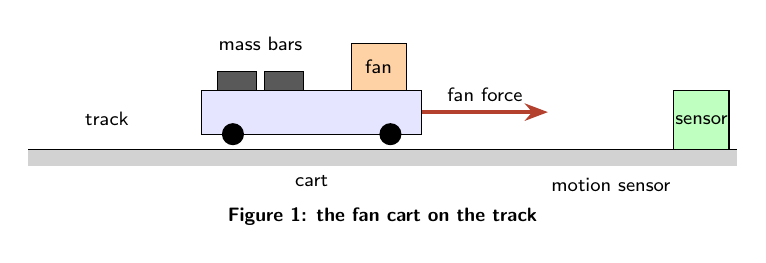
\begin{tikzpicture}[font=\scriptsize]
\fill[gray!35] (0,-0.2) rectangle (9,0); \draw (0,0) -- (9,0);
\draw[fill=blue!10] (2.2,0.2) rectangle (5.0,0.75); \fill (2.6,0.2) circle (0.14); \fill (4.6,0.2) circle (0.14);
\foreach \x in {2.4,3.0} \draw[fill=black!65] (\x,0.75) rectangle (\x+0.5,1.0);
\draw[fill=orange!35] (4.1,0.75) rectangle (4.8,1.35); \node at (4.45,1.05) {fan};
\draw[-{Stealth},very thick,rose] (5.0,0.48) -- (6.6,0.48) node[midway,above,black]{fan force};
\draw[fill=green!25] (8.2,0) rectangle (8.9,0.75); \node at (8.55,0.38) {sensor};
\node[below] at (3.6,-0.2) {cart};\node at (2.95,1.35) {mass bars};\node at (7.4,-0.45) {motion sensor};\node at (1.0,0.4) {track};
\node[font=\scriptsize\bfseries] at (4.5,-0.85) {Figure 1: the fan cart on the track};
\end{tikzpicture}\qquad
\begin{tikzpicture}[font=\scriptsize]
\draw[->] (0,0) -- (6.4,0) node[right]{time (s)}; \draw[->] (0,0) -- (0,4.4) node[above]{speed (m/s)};
\foreach \t in {0,0.5,1.0,1.5,2.0} \draw (\t*3,0.05) -- (\t*3,-0.05) node[below]{\t};
\foreach \s in {0.5,1.0} \draw (0.05,\s*4) -- (-0.05,\s*4) node[left]{\s};
\fill (0,0) circle (0.06);
\fill (1.5,0.84) circle (0.06);
\fill (3,1.76) circle (0.06);
\fill (4.5,2.64) circle (0.06);
\fill (6,3.52) circle (0.06);
\draw[dashed,rose] (1.5,0) -- (1.5,4.1) node[above]{marker 1}; \draw[dashed,rose] (4.5,0) -- (4.5,4.1) node[above]{marker 2};
\node[font=\scriptsize\bfseries] at (3,-1.1) {Figure 2: speed graph, one run};
\end{tikzpicture}
\end{center}
\begin{center}
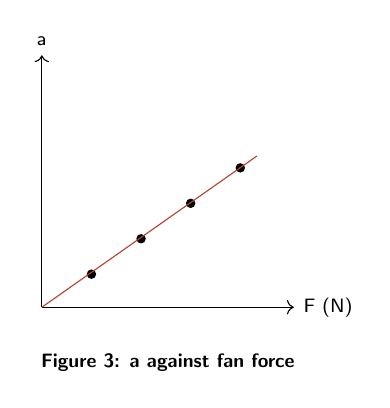
\begin{tikzpicture}[font=\scriptsize,scale=1]
\draw[->] (0,0) -- (3.2,0) node[right]{F (N)}; \draw[->] (0,0) -- (0,3.2) node[above]{a};
\fill (0.630,0.420) circle (0.06);
\fill (1.260,0.870) circle (0.06);
\fill (1.890,1.320) circle (0.06);
\fill (2.520,1.770) circle (0.06);
\draw[rose] (0,0) -- (2.73,1.92);
\node[font=\scriptsize\bfseries] at (1.6,-0.7) {Figure 3: a against fan force};
\end{tikzpicture}\qquad
\begin{tikzpicture}[font=\scriptsize]
\draw[->] (0,0) -- (3.2,0) node[right]{m (kg)}; \draw[->] (0,0) -- (0,3.2) node[above]{a};
\fill (0.750,2.640) circle (0.06);
\fill (1.125,1.770) circle (0.06);
\fill (1.500,1.320) circle (0.06);
\fill (2.250,0.870) circle (0.06);
\draw[rose] plot[smooth] coordinates {(0.75,2.64)(1.125,1.77)(1.5,1.32)(2.25,0.87)};
\node[font=\scriptsize\bfseries] at (1.6,-0.7) {Figure 4: a against mass};
\end{tikzpicture}\qquad
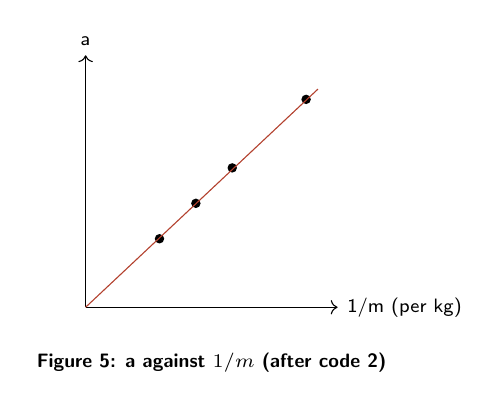
\begin{tikzpicture}[font=\scriptsize]
\draw[->] (0,0) -- (3.2,0) node[right]{1/m (per kg)}; \draw[->] (0,0) -- (0,3.2) node[above]{a};
\fill (0.938,0.870) circle (0.06);
\fill (1.400,1.320) circle (0.06);
\fill (1.862,1.770) circle (0.06);
\fill (2.800,2.640) circle (0.06);
\draw[rose] (0,0) -- (2.95,2.77);
\node[font=\scriptsize\bfseries] at (1.6,-0.7) {Figure 5: a against $1/m$ (after code 2)};
\end{tikzpicture}
\end{center}
\textbf{The fan cart on the track}\par \textit{Axes.} None: this is a picture. \textit{One mark.} Each part is labeled: fan, cart, bars on top, track, motion sensor at the far end, force sensor on the fan. \textit{Look first.} The fan on top of the cart and the bars sitting on the cart. \textit{Wrong reading.} Thinking something pulls the cart: nothing pulls it, the fan pushes it.\par\medskip
\textbf{The speed graph from one run}\par \textit{Axes.} Across: time in seconds, 0 to 2.0. Up: speed in m/s. \textit{One mark.} One dot is one reading of the cart's speed at one moment. \textit{Look first.} Whether the dots climb in a straight line, and how steep it is. \textit{Wrong reading.} Reading the height of the last dot as the acceleration: that is the final speed. Acceleration is how much the speed grows each second.\par\medskip
\textbf{Acceleration against fan force (Part 1)}\par \textit{Axes.} Across: fan force in N. Up: acceleration in m/s\textsuperscript{2}. \textit{One mark.} One dot is one run: the fan force and the acceleration it gave. \textit{Look first.} Do the dots climb, and do they sit near a straight line? \textit{Wrong reading.} Reading a dot's height as a fan force: height is acceleration.\par\medskip
\textbf{Acceleration against mass (Part 2)}\par \textit{Axes.} Across: mass in kg. Up: acceleration in m/s\textsuperscript{2}. \textit{One mark.} One dot is one run at one mass, with the fan force fixed. \textit{Look first.} Do the dots fall, and do they fall straight or bend? \textit{Wrong reading.} Calling it a straight line because the first two dots look straight: look at all four.\par\medskip
\textbf{Acceleration against 1/m} (after code 2)\par \textit{Axes.} Across: 1/m, which is one divided by the mass, in per kg. Up: acceleration in m/s\textsuperscript{2}. \textit{One mark.} One dot is one run: its 1/m and its acceleration. \textit{Look first.} Do the dots sit on a straight line that passes through the corner? \textit{Wrong reading.} Reading 1/m as the mass: a heavy cart has a small 1/m.\par\medskip

\section{The data (every number is author-set; the formula stays in the engine)}
The engine uses $a=(F-f)/m$ with $f=0.01\,\mathrm{N}$ of track drag. No student screen shows it. Fan force 0.15 N per setting. Cart 0.5 kg. Each bar 0.25 kg. Run 2.0 s. Tolerance for a reading: the larger of 10\% or 0.03 \ensuremath{\mathrm{m/s^2}}.
\begin{center}\begin{tabular}[t]{@{}c c c c@{}}\toprule \multicolumn{4}{c}{Part 1: mass fixed (2 bars)}\\ setting & $F$ (N) & $m$ (kg) & $a$ (\ensuremath{\mathrm{m/s^2}})\\\midrule
1 & 0.15 & 1.00 & 0.14 \\
2 & 0.30 & 1.00 & 0.29 \\
3 & 0.45 & 1.00 & 0.44 \\
4 & 0.60 & 1.00 & 0.59 \\
\bottomrule\end{tabular}\qquad\begin{tabular}[t]{@{}c c c c c@{}}\toprule \multicolumn{5}{c}{Part 2: fan setting 3}\\ bars & $m$ (kg) & $F$ (N) & $a$ (\ensuremath{\mathrm{m/s^2}}) & $1/m$\\\midrule
0 & 0.50 & 0.45 & 0.88 & 2.00 \\
1 & 0.75 & 0.45 & 0.59 & 1.33 \\
2 & 1.00 & 0.45 & 0.44 & 1.00 \\
4 & 1.50 & 0.45 & 0.29 & 0.67 \\
\bottomrule\end{tabular}\end{center}
Test run (after code 2): 3 bars, 1.25 kg, expected $a=0.35$ \ensuremath{\mathrm{m/s^2}} (on the $1/m$ line, $1/m=0.80$). \textbf{Wording on every screen:} “about double” and “about half”, never “exactly”. The force doubling gives 2.07 and 2.03 because of the tiny drag. Mr.\ D names that drag at huddle 2.

\section{Item bank (Checks tab)}
Three hidden bands. The top band is the standard. Bold is the correct option. Numeric answers show the accepted range.
\begin{longtable}{@{}p{0.4in} p{4.7in} p{1.2in}@{}}\toprule \textbf{Id} & \textbf{Item} & \textbf{Answer}\\\midrule\endhead
b1-1 & Two carts start at rest. Speed graph A reaches 1.2 m/s after 2.0 s. Speed graph B reaches 0.6 m/s after 2.0 s. Which cart has the bigger acceleration? \newline \textbf{A. Cart A} \newline B. Cart B \newline C. They are the same & option A \\
b1-2 & A cart's speed grows from 0 to 1.20 m/s in 2.0 s. What is its acceleration? & 0.60 $\pm$ 0.03 \ensuremath{\mathrm{m/s^2}} \\
b1-3 & A 1.00 kg cart is run at fan force 0.15 N and then at 0.30 N. The acceleration goes from 0.14 to 0.29 m/s\textsuperscript{2}. About how many times bigger is the acceleration? \newline A. about half \newline B. about the same \newline \textbf{C. about 2 times} \newline D. about 4 times & option C \\
b1-4 & The fan force stays at 0.45 N. The mass goes from 0.50 kg to 1.00 kg. The acceleration goes from 0.88 to 0.44 m/s\textsuperscript{2}. What happened to the acceleration when the mass doubled? \newline A. It about doubled \newline B. It stayed the same \newline \textbf{C. It about halved} \newline D. It about quadrupled & option C \\
b2-1 & A fan force of 0.15 N gave a 1.00 kg cart 0.14 m/s\textsuperscript{2}. A force of 0.30 N gave it 0.29 m/s\textsuperscript{2}. Predict the acceleration for a force of 0.60 N. & 0.58 $\pm$ 0.04 \ensuremath{\mathrm{m/s^2}} \\
b2-2 & The fan force stays the same. A 0.75 kg cart accelerates at 0.59 m/s\textsuperscript{2}. Predict the acceleration of a 1.50 kg cart. & 0.30 $\pm$ 0.03 \ensuremath{\mathrm{m/s^2}} \\
b2-3 & Part 1: acceleration on the up axis, fan force across, mass fixed. Which picture shows the shape of your data? \newline \textbf{A. rising straight line from near the corner} \newline B. falling curve \newline C. flat line & option A \\
b2-4 & Part 2: acceleration on the up axis, mass across, fan force fixed. Which picture shows the shape of your data? \newline A. rising straight line \newline \textbf{B. falling curve, steep then flatter} \newline C. falling straight line & option B \\
b3-1 & A 1.00 kg cart at 0.30 N accelerates at 0.29 m/s\textsuperscript{2}. A stronger fan makes the force 0.60 N and the cart is loaded to 2.00 kg. Predict the new acceleration. & 0.29 $\pm$ 0.03 \ensuremath{\mathrm{m/s^2}} \\
b3-2 & Which sentence do the Part 1 and Part 2 data support? \newline \textbf{A. Doubling the fan force about doubles the acceleration, and doubling the mass about halves it.} \newline B. Doubling the fan force about halves the acceleration, and doubling the mass about doubles it. \newline C. Doubling the fan force about doubles the acceleration, and doubling the mass changes nothing. \newline D. Doubling the fan force or doubling the mass about doubles the acceleration. & option A \\
b3-3 & The fan force stays at 0.45 N. A 0.50 kg cart accelerated at 0.88 m/s\textsuperscript{2} and a 1.00 kg cart at 0.44 m/s\textsuperscript{2}. Predict the acceleration of a 2.00 kg cart. & 0.22 $\pm$ 0.03 \ensuremath{\mathrm{m/s^2}} \\
b3-4 & A student says: "The fan force was the same 0.45 N for the 0.50 kg cart and the 1.50 kg cart, so their accelerations should match." What do the data say? \newline \textbf{A. The 1.50 kg cart had about one third the acceleration (0.29 versus 0.88 m/s\textsuperscript{2}), so the same force does not give the same acceleration.} \newline B. The student is right: the same force gives the same acceleration. \newline C. The 1.50 kg cart had about three times the acceleration. \newline D. The 1.50 kg cart had about half the acceleration. & option A \\
\bottomrule\end{longtable}
Each item has three hints: 1 points to the step card, 2 does the first step, 3 shows the same move on another example. No hint gives the answer. Each costs a fresh attempt. Generators (teacher key shows two samples per band here, three in the data file):
\begin{longtable}{@{}p{0.6in} p{4.7in} p{1.1in}@{}}\toprule
band 1 & A cart's speed grows from 0 to 0.60 m/s in 3.0 s. What is its acceleration? & 0.20 \ensuremath{\mathrm{m/s^2}} \\
band 1 & A cart's speed grows from 0 to 1.80 m/s in 3.0 s. What is its acceleration? & 0.60 \ensuremath{\mathrm{m/s^2}} \\
band 2 & A fan force of 0.30 N gives a 1.00 kg cart an acceleration of 0.29 m/s\textsuperscript{2}. Predict the acceleration for a fan force of 0.90 N on the same cart. & 0.87 \ensuremath{\mathrm{m/s^2}} \\
band 2 & A fan force of 0.15 N gives a 1.00 kg cart an acceleration of 0.14 m/s\textsuperscript{2}. Predict the acceleration for a fan force of 0.30 N on the same cart. & 0.28 \ensuremath{\mathrm{m/s^2}} \\
band 3 & A 0.75 kg cart with a fan force of 0.15 N accelerates at 0.19 m/s\textsuperscript{2}. A stronger fan makes the force 4 times bigger, and the cart is loaded to 3 times the mass. Predict the new acceleration. & 0.25 \ensuremath{\mathrm{m/s^2}} \\
band 3 & A 0.50 kg cart with a fan force of 0.15 N accelerates at 0.28 m/s\textsuperscript{2}. A stronger fan makes the force 2 times bigger, and the cart is loaded to 3 times the mass. Predict the new acceleration. & 0.19 \ensuremath{\mathrm{m/s^2}} \\
\bottomrule\end{longtable}

\section{Huddle 2: the script (the most important block)}
\textbf{State what is tested.} What will be tested: say how acceleration changes when the fan force doubles and when the mass doubles, using numbers from a table. Read a straight line to predict a new acceleration.\par
\textbf{Blanks on the formalizing tab.} Double the fan force, same cart: the acceleration is about \_\_\_\_\_\_. (double) \quad Double the mass, same fan force: the acceleration is about \_\_\_\_\_\_. (half) \quad Acceleration against 1/m is a \_\_\_\_\_\_ line through the corner. (straight)\par
\textbf{Three worked problems} (Mr.\ D draws them; the site shows the answers afterward):
\begin{description}[leftmargin=2em]
\item[\textbf{W1}] A 1.00 kg cart at fan force 0.15 N has acceleration 0.14 m/s\textsuperscript{2}. Predict the acceleration at 0.45 N.\par 0.45 N $\div$ 0.15 N = 3 times the force. \quad 3 $\times$ 0.14 m/s\textsuperscript{2} = 0.42 m/s\textsuperscript{2}. \quad Check: your table says about 0.44. Close.
\item[\textbf{W2}] A 0.50 kg cart at 0.45 N has acceleration 0.88 m/s\textsuperscript{2}. Predict the acceleration of a 1.50 kg cart at 0.45 N.\par 1.50 kg $\div$ 0.50 kg = 3 times the mass. \quad Three times the mass gives one third the acceleration. \quad 0.88 m/s\textsuperscript{2} $\div$ 3 = 0.29 m/s\textsuperscript{2}.
\item[\textbf{W3}] On your acceleration-against-1/m line, 1/m = 1.00 per kg gives 0.44 m/s\textsuperscript{2}. Predict the acceleration of a 1.25 kg cart.\par 1/m = 1 $\div$ 1.25 kg = 0.80 per kg. \quad The line passes through the corner, so 0.80 gives 0.80 $\times$ 0.44 m/s\textsuperscript{2}. \quad 0.80 $\times$ 0.44 = 0.35 m/s\textsuperscript{2}.
\end{description}
\textbf{Three crux questions} (these are on the test): 1. Same cart, the fan force triples. About how many times bigger is the acceleration? \textit{about 3 times.} 2. Same fan force, the mass triples. What happens to the acceleration? \textit{it becomes about one third.} 3. Which of your graphs are straight lines? \textit{acceleration against fan force, and acceleration against 1/m. Not acceleration against mass.}\par
\textbf{Mr.\ D says}: friction: the track has a tiny drag. That is why the force line misses the corner by a hair. 1/m: one divided by the mass. Per kg.\par
\textbf{Do not say} “second law”, “proportional”, “inverse”, “slope” or “newton”. Then give code 2.

\section{CER and exit ticket}
\textbf{CER prompt.} How does the cart's acceleration change when the fan force doubles? When the mass doubles? Use numbers from your tables. Checklist: My claim answers both parts: the fan force and the mass. My evidence has two numbers from Part 1 and two from Part 2. I say about double and about half, not exactly. My reasoning says why the numbers point to my claim.\par
\begin{tabularx}{\linewidth}{@{}l Y c@{}}\toprule \textbf{Criterion} & \textbf{What earns the point} & \textbf{circle}\\\midrule
Claim & Answers both parts: the fan force and the mass. & 0\quad 1\\
Evidence & Two numbers from Part 1 and two from Part 2. Their own values; ignore numbers under 0.1 that match by luck. & 0\quad 1\\
Reasoning & Says why the numbers point to the claim, with about double and about half. & 0\quad 1\\
\bottomrule\end{tabularx}
\textbf{Exit ticket (drawing on paper).} Draw two small graphs, both with acceleration going up. On the first put fan force across. On the second put mass across, with the fan force fixed. Sketch the dots and label the axes.\par
\textbf{Look for:} first graph: dots climb in a straight line from near the corner; second graph: dots fall, steep at first and then flatter; axes labeled with the quantity on each.

\section{Teacher side and record}
The teacher key shows every item next to the lesson, three generated problems per band, every lab-record row, the three predictions (pre-lab, before Part 2, the test) with the choice or typed value, and the CER with the count check. Scores stay on the student's own device (\texttt{MrD.profile.record}). No end-of-lesson stamp, no report code. Two huddle codes. The projector page is the questions plus room to draw.

\section{Paper fallback (rule 14)}
If Chromebooks fail, print these cards. The student reads $a=(v_{2.0}-v_0)/2.0$ and fills the same two tables. Card T-1 goes out only after code 2. Speeds in m/s from seeds 700 to 708.
\begin{center}\small\begin{tabular}{@{}l l c c c c c c c@{}}\toprule card & part & $F$ (N) & $m$ (kg) & 0 s & 0.5 s & 1.0 s & 1.5 s & 2.0 s\\\midrule
P1-1 & Part 1 & 0.15 & 1.00 & 0.00 & 0.06 & 0.13 & 0.22 & 0.28 \\
P1-2 & Part 1 & 0.30 & 1.00 & 0.00 & 0.15 & 0.29 & 0.43 & 0.58 \\
P1-3 & Part 1 & 0.45 & 1.00 & 0.00 & 0.21 & 0.44 & 0.66 & 0.88 \\
P1-4 & Part 1 & 0.60 & 1.00 & 0.00 & 0.29 & 0.59 & 0.87 & 1.18 \\
P2-1 & Part 2 & 0.45 & 0.50 & 0.00 & 0.43 & 0.89 & 1.33 & 1.77 \\
P2-2 & Part 2 & 0.45 & 0.75 & 0.00 & 0.29 & 0.58 & 0.87 & 1.17 \\
P2-3 & Part 2 & 0.45 & 1.00 & 0.00 & 0.23 & 0.44 & 0.65 & 0.87 \\
P2-4 & Part 2 & 0.45 & 1.50 & 0.00 & 0.16 & 0.29 & 0.45 & 0.59 \\
T-1 & test (after code 2) & 0.45 & 1.25 & 0.00 & 0.20 & 0.37 & 0.53 & 0.70 \\
\bottomrule\end{tabular}\end{center}

\section{Open decisions for Mr.\ D}
\begin{enumerate}
\item \textbf{Code 2 and unfinished tables.} Default here: code 2 is never blocked. Confirm.
\item \textbf{Where the 10-minute huddle change lives.} Huddle 1 here is 8 minutes. The repo has 18 and 32 in \texttt{shared/pace.js}; the change is not on main.
\item \textbf{Calculator and units.} No calculator tutorial is needed today: the only arithmetic is dividing by 2.0 and the ratio rules.
\item \textbf{The $1/m$ word.} It appears only after code 2. Mr.\ D says “one over m” once in huddle 2.
\item \textbf{Three bands in the repo.} The repo's four-band standard and \texttt{check-lessons --strict} are still open (DAY-RULES).
\end{enumerate}
\end{document}
